\chapter{Нестационарная теория возмущений}

\section{Нестационарное возмущение дискретного спектра. Переходы под влиянием возмущения, действующего в течение конечного времени}

Рассматривается общая задача теории возмущений, когда гамильтониан физической системы можно записать в виде
$$
\op{H} = \op{H}^\zr + \op{V}(t),
$$
где $\op{V}(t)$ в известном выше смысле мало. Теперь мы считаем, что возмущение зависит от времени. Зависимость гамильтониана от времени характерна для незамкнутых систем, т.~е. там, где действуют внешние силы. Например, взаимодействие квантовой системы с электромагнитной волной.

Считаем, что возмущение действует в течение некоторого \underline{конечного} промежутка времени $T$:
$$
\op{V}(t) = \left \{ 
  \begin{matrix}
    \op{w}(t), &  0 < t < T \\
    0, & t \le 0, t \ge T
  \end{matrix}
  \right .
$$

Строго говоря, у такой системы \underline{нет} стационарных состояний, и говорить о поправках к собственным значениям энергии в этом случае \underline{нельзя}. Но если есть малый параметр (как в главе \rom{12}, он полагается включенным в $\op{V}$), то можно применить идеологию метода ТВ для приближенного вычисления волновых функций.

Пусть при $\op{V}(t) = 0$ ($t \le 0$) у системы существуют стационарные состояния с дискретным спектром, т.~е.
$$
i \hbar \pd{}{t} \ket{\psi_n^\zr(t)} = \op{H}^\zr \ket{\psi_n^\zr(t)} 
$$
$$
\ket{\psi_n^\zr (t)} = e^{-i \frac{E_n^\zr t}{\hbar}} \ket{\psi_n^\zr},
$$
где $\op{H}^\zr \ket{\psi_n^\zr} = E_n^\zr \ket{\psi_n^\zr}$ (см.~\sref{4}{1}). Обозначим $\hbar \omega_n = E_n^\zr$. Тогда общее решение невозмущенного уравнения может быть записано в виде
$$
\ket{\psi^\zr(t)} = \sum_k c_k \ket{\psi_k^\zr (t)} = \sum_k c_k e^{-i \omega_k t} \ket{\psi_k^\zr},
$$
где, как обычно, $c_k$ --- коэффициенты разложения в линейную суперпозицию, квадраты модулей которых --- вероятности обнаружить систему в стационарном состоянии <<k>>.

\subsection{Метод вариации постоянных}

Учтем теперь наличие $\op{V}(t)$, считая, что $c_k \equiv c_k(t)$. Поскольку ${w_k(t) \equiv \abs{c_k(t)}^2}$, то вероятность обнаружить систему в состоянии <<k>> становится функцией времени, и можно описать переходы из одного состояния в другое. Итак, будем искать решение возмущенного уравнения
\begin{equation}
\label{eq:13_1_1}
i \hbar \pd{}{t} \ket{\psi(t)} = (\op{H}^\zr + \op{V}(t)) \ket{\psi(t)}
\end{equation}
в виде суммы
\begin{equation}
\label{eq:13_1_2}
\ket{\psi(t)} = \sum_k c_k(t) \ket{\psi_k^\zr(t)}
\end{equation}

Подставим разложение \eqref{eq:13_1_2} в уравнение \eqref{eq:13_1_1}:
$$
i \hbar \sum_k \brc{\dot{c_k} \ket{\psi_k^\zr (t) } + c_k \cancel{\pd{}{t} \ket{\psi_k^\zr (t)}}} = \sum_k c_k \brc{ \cancel{\op{H}^\zr \ket{\psi_k^\zr(t)}} + \op{V} \ket{\psi_k^\zr(t)}}
$$

Помня, что $\ket{\psi_k^\zr(t)}$ удовлетворяют невозмущенному уравнению, получим
\begin{equation}
\label{eq:13_1_3}
i \hbar \sum_k \dot{c_k} \ket{\psi_k^\zr (t)} = \sum_k c_k \op{V}(t) \ket{\psi_k^\zr(t)}
\end{equation}

Проектируем \eqref{eq:13_1_3} на $\bra{\psi_m^\zr(t)}$ и с учетом ортонормировки $\bk{\psi_m^\zr(t)}{\psi_k^\zr(t)} = \delta_{mk}$ имеем:
\begin{equation}
\label{eq:13_1_4}
\boxed{i\hbar \dot{c_m} = \sum_k c_k (t) V_{mk}(t) e^{i \omega_{mk} t}},
\end{equation}
где $\omega_{mk} = \dfrac{(E_m^\zr - E_k^\zr)}{\hbar}$, $V_{mk} = \bfk{\psi_m^\zr}{\op{V}(t)}{\psi_k^\zr}$ --- при зависящем явно от времени $\op{V}$ величины $V_{mk}$ тоже являются функциями времени. Отметим, что нами получено точное соотношение. Для решения этого дифференциального уравнения в общем случае необходима аппроксимация. 

\subsection{Приближение или метод Дирака (1927 г.)}

Считается, что $c_k(t)$ можно представить в виде ряда убывающих функций времени:
$$
c_k(t) = c_k^\zr(t) + c_k^\one(t) + \dots 
$$

Предположим, что возмущение было включено в момент времени $t = 0$. До этого было $\op{H} \equiv \op{H}^\zr$, и система достоверно находилась в состоянии с $E = E_n^\zr$, т.~е.
$$
\boxed{c_k(0) = c_k^\zr(0) = c_k^\zr = \delta_{kn}}
$$
или $c_n^\zr = 1$, $c_k^\zr = 0$ при $k \neq n$ (в нулевом приближении зависимости от времени нет). Тем самым мы поставили начальное условие. Дальнейшее решение приводит к цепочке уравнений в каждом порядке $s$ для $c_m^{(s)}(t)$. Подставляя ряд для $c_k(t)$ в уравнение \eqref{eq:13_1_4}:
$$
i \hbar \pd{}{t} \brcr{\cancel{c_{nm}^\zr} + c_{nm}^\one (t) + \dots} = \sum_k V_{mk} e^{i \omega_{mk} t} \cdot \brcr{\underbrace{c_{nk}^\zr}_{\delta_{nk}} + \underbrace{\cancel{c_{nk}^\one}}_{\text{2й порядок малости}} + \dots}
$$

К каждой из невозмущенных функций вычисляется поправка.

В первом порядке теории возмущений получаем:
\begin{equation}
\label{eq:13_1_5}
\boxed{i \hbar \pd{}{t} c_{nm}^\one = V_{mn}(t) e^{i \omega_{mn} t}}
\end{equation} 
или, что то же самое,
\begin{equation*}
\boxed{c_{nm}^\one = \frac{1}{i\hbar} \int_0^t dt' V_{mn}(t') e^{i \omega_{mn} t'}}, ~~~(0 < t < T)
\end{equation*}

Найденная нами $c_{nm}^\one$ есть поправка 1-го порядка к $n$-ому стационарному состоянию (в нем система находилась до включения возмущения). Дальнейшие вычисления приведут к поправкам высших порядков ТВ. Мы ограничимся первым порядком.

\section{Вероятность перехода}

Какой смысл имеет функция $c_{mn}^\one (t)$? Общее решение имеет вид:
$$
\ket{\psi_n(t)} = \sum_m c_{nm}(t) e^{-i \omega_m t} \ket{\psi_m^\zr}
$$
и про него известно, что

а) \underline{при $t \le 0$:} $c_{nm} = c_{nm}^\zr = \delta_{nm}$, т.~е. система достоверно находилась в состоянии с $E=E_n^\zr$ и в сумме по $m$ есть только одно слагаемое с $m = n$;

б) \underline{при $t > 0$:} действует возмущение. В результате коэффициенты $c_{nm}(t)$ при $m \neq n$, сначала равные нулю, становятся отличными от нуля: $c_{nm}^\one(t) \neq 0$. В соответствии с \underline{принципом линейной суперпозиции состояний} $\boxed{\abs{c_{nm}^\one (t)}^2 = P_{nm}(t)}$ есть вероятность обнаружить систему в момент времени $t$ в состоянии <<m>>, если в начальный момент времени она была в состоянии <<n>> дискретного спектра невозмущенной задачи. Таким образом, в результате действия возмущения может произойти квантовый переход из одного стационарного состояния в другое.

Введем терминологию: $P_{nm}(t)$ --- вероятность этого квантового перехода из состояния <<n>> в состояние <<m>> за время $t$. 

Ранее предполагалось, что возмущение действовало в течение некоторого конечного промежутка времени $T$ (от $t = 0$ до $t = T$ (или $t$)). Строго говоря, все это время система была нестационарной. Только после снятия возмущения система перейдет с той или иной вероятностью к одному из стационарных состояний. При условии малости $\op{V}$ и $T$ говорят о дискретных переходах между стационарными состояниями. Следовательно,  
$$
P_{nm}(t) =\frac{1}{\hbar^2} \left | \int_0^t dt' V_{mn}(t') e^{i \omega_{mn} t'} \right |^2, ~~~0 < t < T
$$

При $-\infty < t < \infty$
$$
P_{nm} = \frac{1}{\hbar^2} \left | \int_{-\infty}^\infty dt' V_{mn}(t')e^{i \omega_{mn}t'} \right |^2 = \boxed{\frac{(2\pi)^2}{\hbar^2} \left | V_{mn}(\omega_{mn})\right|^2} = P_{nm},
$$
где $V_{mn}(\omega_{mn}) = \dfrac{1}{2\pi} \int \limits_{-\infty}^\infty dt' V_{mn}(t') e^{i\omega_{mn}t'}$ --- компонента Фурье матричного элемента $V_{mn}(t)$ оператора возмущения $\op{V}(t)$, действующего в течение конечного промежутка времени.

\section{Адиабатические и внезапные возмущения}

Здесь речь пойдет о промежутках времени, непосредственно примыкающих к моментам включения и выключения возмущения (см. \autoref{fig:13_1}).
\begin{figure}[h!]
\centering
\begin{tikzpicture}[domain=-1:5]
    \draw[->] (-1,0) -- (5,0) node[right] {$t$};
    \draw[->] (0,-0.6) -- (0,3) node[above] {$V(t)$};
	\draw [domain=0:0.2, samples=50] plot (\x, 25 * \x^2);
	\draw [domain=0.2:0.4, samples=50] plot (\x, -25 * \x^2 + 20 *\x - 2);
	\draw [domain=2.6:2.8, samples=50] plot (\x, -25 * \x^2 + 130 *\x - 167);
	\draw [domain=2.8:3, samples=50] plot (\x,  25 *\x^2- 150 * \x + 225);
	\draw [domain=0.4:2.6, samples=50] plot (\x, 2);
    \draw (3.1,0) -- (3.1,-0.6);
    \draw [<->](0,-0.6) -- (3.1,-0.6);	
    \node[below] at (1.5, -0.7) {$T$};	
	\draw[thick] (-1,0) -- (0,0);
	\draw[thick] (3,0) -- (3.7,0);
	\draw[dashed] (0.2,1) -- (0.2,0) node [below] {$t^*$} ;
	\draw[dashed] (0.4,2) -- (0.4,0) node [above] {$\tau$} ;
	\draw[dashed] (2.6,2) -- (2.6,0);
	\node at (2.5, -0.2) {$T-\tau$}; 
\end{tikzpicture}
\caption{Изменения возмущения во времени. $T$ - длительность возмущения, $\tau$ - время включения, $t^*$ - точка перегиба.} \label{fig:13_1}
\end{figure}

\subsection{Адиабатическое изменение возмущения}

Преобразуем интеграл:
\begin{eqnarray*}
\frac{1}{i\hbar} \int_0^T dt' V_{mn}(t')e^{i\omega_{mn}t'} = -\left. \frac{V_{mn}(t')e^{i \omega_{mn}t'}}{\hbar \omega_{mn}}\right|_0^T + \int_0^T dt' \D{V_{mn}(t')}{t'} \frac{e^{i\omega_{mn}t'}}{\hbar \omega_{mn}}
\end{eqnarray*}

Учитывая, что $V_{mn}(0) = V_{mn}(T) = 0$, получим:
\begin{equation}
\label{eq:13_3_1}
P_{nm}(T) = \frac{1}{(\hbar \omega_{mn})^2} \left| \int_0^T dt' \D{V_{mn}(t')}{t'} e^{i\omega_{mn}t'}\right|^2
\end{equation}

\begin{defn}
Матричный элемент оператора возмущения $V_{mn}(t')$ изменяется адиабатически (медленно), если за характерное время переходов в квантовой системе $T_{mn} = \dfrac{2\pi}{\omega_{mn}}$ изменение $V_{mn}$ мало по сравнению с самой величиной $|V_{mn}(t')|$, т.~е.
\end{defn}
\begin{equation}
\label{eq:13_3_2}
\Delta V_{mn}  \simeq T_{mn} \left| \D{V_{mn}}{t'}\right| \ll |V_{mn}|
\end{equation}

Если $\tau$ --- характерное время включения (или выключения) возмущения, то
$$
\Delta V_{mn} \sim T_{mn} \frac{|V_{mn}|}{\tau} \ll |V_{mn}| 
$$
или
$$
\boxed{\frac{T_{mn}}{\tau} \ll 1}
$$
--- {\em условие адиабатичности} (медленности) изменения матричного элемента $V_{mn}$. При этом множитель $\D{V_{mn}}{t'}$ в \eqref{eq:13_3_1} мало меняется по сравнению с экспонентой $e^{i\omega_{mn} t'}$, и его можно (в некоторой точке $t' = t^*$, см. \autoref{fig:13_1}) вынести за знак интеграла, который затем легко берется:
%\begin{gather*}
%\to \omega_{mn} \tau \gg 1 
%\end{gather*}
$$
P_{nm}(T) = \left| \D{}{t'} V_{mn}(t')\right|_{t' = t^*}^2 \brc{\frac{2}{\hbar \omega_{mn}^2}}^2 \sin^2 \brc{\frac{\omega_{mn}T}{2}}
$$

С другой стороны, $|\Delta V_{mn}| \ll \hbar \omega_{mn}$, поэтому неравенство \eqref{eq:13_3_2} можно переписать в виде
\begin{equation}
\label{eq:13_3_3}
\frac{1}{\omega_{mn}} \left| \D{V_{mn}}{t'}\right|_{t' = t^*} \ll \hbar \omega_{mn}
\end{equation}

С учетом условия \eqref{eq:13_3_3} получаем: $\boxed{P_{nm}(T) \ll 1}$, т.~е. при \underline{медленном (адиабатическом) включении или выключении} возмущения квантовая система, находившаяся первоначально в невырожденном состоянии с $E_n^\zr$, будет в первом приближении теории возмущений оставаться в нем же.

\subsection{Внезапное включение возмущения}

В этом случае возмущение практически мгновенно изменяется от 0 до $\op{V}$ за время $\tau \ll T_{mn} \sim 1/\omega_{mn}$. Тогда на протяжении указанного промежутка времени $\omega_{mn} \tau \ll 1$ в подынтегральном выражении \eqref{eq:13_3_1} множитель $e^{i\omega_{mn} t'}$ мало меняется по сравнению с $\D{V_{mn}}{t'}$ и может быть вынесен за знак интеграла. Оставшийся сомножитель $\sim \delta(t')$. В результате интегрирования имеем:
\begin{equation}
\label{eq:13_3_4}
\boxed{P_{mn} \simeq \frac{|V_{mn}|^2}{\hbar^2 \omega_{mn}^2}}
\end{equation}

Здесь $|V_{mn}|$ --- максимальное значение матричного элемента возмущения в момент его включения.

Вероятности перехода при внезапных возмущениях можно найти и в тех случаях, когда возмущение не является малым. Если изменение гамильтониана: $\op{H}^\zr \to \op{H}$ происходит за время $\tau \ll \dfrac{1}{\omega_{mn}}$, то волновая функция системы <<не успевает>> измениться и остается той же $\psi_n^\zr$, что и до возмущения. Отвечающий ей волновой вектор $\ket{\psi_n^\zr}$, однако, уже не является СВ нового гамильтониана $\op{H}$, но может быть разложен по полной ортонормированной системе его СВ $\brcr{\ket{\psi_f}}$:
%$$
%  \begin{CD}
%  \op{H}^\zr @>>> \op{H}~~~\text{за время } \tau \ll \frac{1}{\omega_{mn}}\\
%  @VVV                      @VVV\\
%  \psi_n^\zr   @.           \brcr{\ket{\psi_f}}
%  \end{CD}
%$$
$$
\ket{\psi_n^\zr} = \underbrace{\sum_f \ket{\psi_f} \bra{\psi_f}}_{=\op{\mathbf{1}}}\ket{\psi_n^\zr}
$$
и, согласно общим правилам квантовой механики, вероятность перехода $P_{nm}$ системы в новое стационарное состояние <<m>> задается формулой
\begin{equation}
\label{eq:13_3_5}
\boxed{P_{nm} = |\bk{\psi_m}{\psi_n^\zr}|^2}
\end{equation}

(формулу \eqref{eq:13_3_5} можно использовать при решении задачи 9 из 1-го задания \rom{2} семестра)

Если считать возмущение $\op{V}$ малым, то можно показать, что общая формула \eqref{eq:13_3_5} переходит в формулу \eqref{eq:13_3_4} (см.~\llref{41}{3}).

\section{Переходы под влиянием постоянного во времени возмущения. <<Золотое правило>> Ферми}

\begin{figure}[h!]
\centering
\begin{tikzpicture}[domain=-1:5]
    \draw[->] (-1,0) -- (5,0) node[right] {$t$};
    \draw[->] (0,-0.1) -- (0,3) node[above] {$V(t)$};
	\draw[thick] (0,0) -- (0,2);
	\draw[thick] (0,2) -- (3,2);
	\draw[thick] (3,2) -- (3,0) node[below] {$T$};
	\draw[thick] (-1,0) -- (0,0) node [below] {0};
	\draw[thick] (3,0) -- (3.7,0);
\end{tikzpicture}
\caption{Постоянное во времени возмущение} \label{fig:13_2}
\end{figure}

Если возмущение постоянно во времени на промежутке от 0 до $T$ ($V = const$, см. \autoref{fig:13_2}), то из \eqref{eq:13_1_5} следует:
\begin{align*}
P_{nm} = \left| \frac{1}{i \hbar} \int_0^T dt' \Vmn e^{i\ommn t'} \right|^2 
  & = \left|\frac{1}{i\hbar} \Vmn \frac{e^{i \ommn T} - 1}{i\ommn}\right|^2
  = \\ & = \frac{\abs{\Vmn}^2}{\hbar^2} \frac{2 (1 - \cos \ommn T)}{\ommn^2} = \frac{\abs{\Vmn}^2}{\hbar^2} f(\ommn, T)
\end{align*}

Здесь $f(\omega, T) = \dfrac{2(1 - \cos \omega T)}{\omega^2}$ --- {\em спектральная функция} (см. \autoref{fig:13_3}), которая имеет острый пик при $T \to \infty$ шириной $\sim \dfrac{2\pi}{T}$ вблизи $\omega =0$. При $T \to \infty$ присутствует одно из определений $\delta$-функции (см.~\llref{42}{3}):
$$
\lim_{T \to \infty} \brc{\frac{f(\omega, T)}{T}} = 2\pi \delta(\omega)
$$

\begin{figure}[h!]
\centering
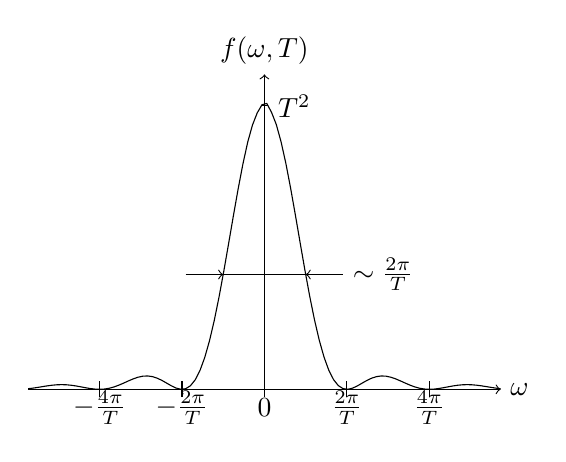
\begin{tikzpicture}[domain=-3:3]
    \draw[->] (-3,0) -- (3,0) node[right] {$\omega$};
    \draw[->] (0,-0.1) -- (0,4) node[above] {$f(\omega, T)$};
    \draw [domain=-3:3, samples=100] plot (\x, {0.2 * (1 - cos((6 * \x) r)) / (\x * \x)});
    \draw[-] (1.047,-0.1) -- (1.047,0.1) node [below]{$\frac{2 \pi}{T}$};
    \draw[-] (-1.047,-0.1) -- (-1.047,0.1) node [below]{$-\frac{2 \pi}{T}$};
    \draw[-] (2.094,-0.1) -- (2.094,0.1) node [below]{$\frac{4 \pi}{T}$};
    \draw[-] (-2.094,-0.1) -- (-2.094,0.1) node [below]{$-\frac{4 \pi}{T}$};
    \draw[-] (-0.05,3.6) -- (0.05,3.6) node [right]{$T^2$};
    \node[below] at (0, 0) {$0$};
    \draw[-] (0.524,1.458) -- (-0.524,1.458);
    \draw[<-] (0.524,1.458) -- (1,1.458) node [right]{$\sim \frac{2 \pi}{T}$};
    \draw[->] (-1,1.458) -- (-0.524,1.458);
\end{tikzpicture}
\caption{График спектральной функции.} \label{fig:13_3}
\end{figure}

Тогда вероятность квантовых переходов в единицу времени есть
\begin{align}
w_{nm} = \left . \frac{P_{nm}}{T}\right|_{T \to \infty} 
  & = \frac{\abs{\Vmn}^2}{\hbar^2} \underbrace{\lim_{T \to \infty} \frac{f(\ommn, T)}{T}}_{2\pi\delta{\ommn}} = \nonumber \\
  & = \frac{\abs{\Vmn}^2}{\hbar^2} 2 \pi \delta \brc{\ommn}
  = \frac{\abs{\Vmn}^2}{\hbar^2} 2 \pi \delta \brc{\frac{E_m - E_n}{\hbar}} = \nonumber \\
  \label{eq:13_4_1}
  &= \boxed {
    \frac{\abs{\Vmn}^2}{\hbar} 2 \pi \delta (E_m - E_n) = w_{nm}
  }
\end{align}

Переход к $\delta$-функции --- идеализация, облегчающая дальнейшие вычисления (в частности, проведение в дальнейшем интегрирования по энергии конечных состояний). Из \autoref{fig:13_3} видно, что квантовые переходы в основном происходят в состояния, энергия которых отличается не более, чем на $\delta E \sim \dfrac{2\pi}{T} \hbar$ --- с такой точностью сохраняется энергия, что связано с соотношением неопределенностей между энергией и временем ее измерения $\Delta t$
\begin{equation}
\label{eq:13_4_2}
\boxed{\Delta E \Delta t \ge \frac{\hbar}{2}} 
\end{equation}

За время $\Delta t$ энергия системы не может быть измерена точнее величины $\Delta E$, определяемой соотношением \eqref{eq:13_4_2}. В частности, если состояние является стационарным ($\Delta t \to \infty$), то энергия микрообъекта будет точно определенной ($\Delta E \to 0$) (см.~\llref{44}{3}).

В полученной формуле \eqref{eq:13_4_1} для вероятности квантовых переходов в единицу времени квантовые числа <<n>> и <<m>> начального и конечного состояний фиксированы. Важное прикладное значение эта формула имеент в следующем случае:
\begin{enumerate}
\item Спектр (по крайней мере, конечных, либо начальных и конечных состояний) --- \underline{непрерывный} (либо квазинепрерывный).
\item Постановка физической задачи такова, что необходимо найти \underline{полную} вероятность квантовых переходов в единицу времени из начального состояния <<n>> в континуальную группу состояний <<m>>, обладающих почти одинаковой энергией и близкими значениями матричных элементов.
\end{enumerate}

\begin{exmpl}
Вероятность упругого рассеяния сталкивающихся частиц в элемент телесного угла $d\Omega_{\vec k}$, $\vec k$ --- волновой вектор конечного состояния (рассеянной волны (частицы)). Здесь роль возмущения играет потенциальная энергия $U(\vr)$ взаимодействия между частицами --- <<борновское приближение>> (см. главу \rom{19} <<Теория рассеяния>> и задачу 7 из 2-го задания \rom{2} семестра).
\end{exmpl}

При такой постановке задачи требуется просуммировать вероятности переходов в единицу времени по квантовым числам <<m>> конечных состояний и учесть непрерывный характер спектра конечных состояний. Последнее означает переход от суммирования к интегрированию в выражении для полной вероятности:
$$
W_n = \sum_m w_{nm} \to \int w_{mn} d \nu_m,
$$
где $d \nu_m$ - число квантовых состояний в интервале энергий $E_m \div E_m + dE_m$: \newline $\boxed{d \nu_m = \rho(E_m) dE_m}$. Множитель $\rho(E_m) = \D{\nu_m}{E_m}$ --- плотность конечных состояний, т.~е. число конечных состояний, приходящихся на единичный интервал энергий вблизи $E_m$. Тогда полная вероятность переходов из начального состояния <<n>> в континуальную группу состояний, близких <<m>> есть 
$$
W_n = \int w_{mn} \rho(E_m)dE_m = \left |_{\eqref{eq:13_4_1}} \dfrac{2\pi}{\hbar} \int \abs{\Vmn}^2 \delta(E_m - E_n) \rho(E_m)dE_m \right .=
$$
\begin{equation}
\label{eq:13_4_3}
= \boxed{ \left. \frac{2\pi}{\hbar} \abs{\Vmn}^2 \rho(E_m) \right|_{E_m = E_n} = W_n}
\end{equation}

Формула \eqref{eq:13_4_3} означает {\em <<золотое правило>> Ферми} --- полная вероятность квантовых переходов в единицу времени не зависит от длительности действия возмущения.

Анализируя \eqref{eq:13_4_3}, приходим к следующим выводам:
\begin{enumerate}
\item При квантовых переходах сохраняется энергия, что выражается $\delta$-функцией. Поскольку $\op{V} = const$, то и сохраняется энергия. Реализуются лишь такие переходы, которые сохраняют энергию. Энергия может только перераспределяться между отдельными частями единой системы. Энергия не изменяется, значит, она --- интеграл движения, но могут изменяться другие характеристики, например, вектор импульса в борновском приближении теории рассеяния.

\item Полученная формула описывает полную вероятность квантовых переходов в единицу времени из начального состояния <<n>> во все состояния <<m>>, обладающие почти одинаковой энергией и близкими значениями матричных элементов. 

\item Если спектр существенно дискретный, то нельзя переходить ${P_{nm} \to W_n}$. Для этого нужно, чтобы $f(\ommn, T)$ была $\delta$-функцией по сравнению с $\rho(E_m)$ (см. \autoref{fig:13_4}). 
\end{enumerate}

\begin{figure}[h!]
\centering
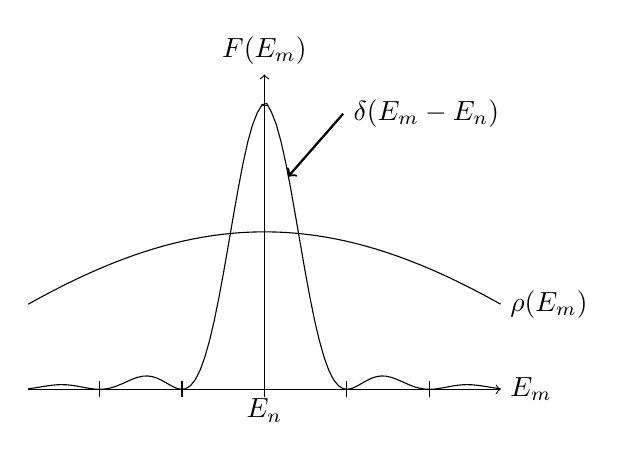
\begin{tikzpicture}[domain=-3:3]
    \draw[->] (-3,0) -- (3,0) node[right] {$E_m$};
    \draw[->] (0,-0.1) -- (0,4) node[above] {$F(E_m)$};
    \draw [domain=-3:3, samples=100] plot (\x, {0.2 * (1 - cos((6 * \x) r)) / (\x * \x)});
    \draw[-] (1.047,-0.1) -- (1.047,0.1) ;
    \draw[-] (-1.047,-0.1) -- (-1.047,0.1) ;
    \draw[-] (2.094,-0.1) -- (2.094,0.1) ;
    \draw[-] (-2.094,-0.1) -- (-2.094,0.1) ;
    \draw[-] (-0.05,3.6) -- (0.05,3.6) ;
    \node [below] at (0, 0) {$E_n$};
	\draw[<-, thick] (0.3, 2.7) -- (1, 3.5) node [right] {$\delta(E_m - E_n)$};   
    %\draw[<-, thick] (0.85, 0.2) -- (1.5, 0.5) node [right] {$\delta(E_m - E_n)$};
    \draw [domain=-3:3, samples=50] plot (\x, {2 * cos((\x / 3) r)}) node [right] {$\rho(E_m)$};
\end{tikzpicture}
\caption{К применимости \eqref{eq:13_4_3}.} \label{fig:13_4}
\end{figure}

\section{Переходы под действием периодического возмущения в дискретном и непрерывном спектрах}

В силу эрмитовости $\op{V}$ оператор периодического во времени возмущения может быть представлен в виде
\begin{equation}
\label{eq:13_5_1}
\op{V}(t) = \op{V}e^{-i\omega t} + \op{V}^\dag e^{i\omega t},
\end{equation}
где $\op{V}$ не зависит от времени, а $\op{V}(t)$, как и в \S 4, действует на промежутке $[0, T]$. Тогда подставляя \eqref{eq:13_5_1} в выражение \eqref{eq:13_1_5} для коэффициентов $c_{nm}^\one (t)$ общей теории, будем иметь:
\begin{gather*}
c_{nm}^\one = \frac{1}{i \hbar} \int_0^T dt \brcr{\Vmn e^{i(\ommn - \omega)t} + \underbrace{\Vmn^\dag}_{V_{nm}^*} e^{i(\ommn + \omega)t}} = \\
= \frac{\Vmn [e^{i(\ommn - \omega)T} - 1]}{i \hbar i (\ommn - \omega)} + \frac{\Vmn^\dag [e^{i(\ommn + \omega)T} - 1]}{i \hbar i (\ommn + \omega)}
\end{gather*}

При $\omega \to \pm \ommn = \pm (E_m - E_n) / \hbar$ ({\em резонансный случай}), основной вклад в вероятность переходов вносит либо первое, либо второе слагаемое. При этом продолжая вычисления, аналогичные случаю $\op{V} = const$ предыдущего \S 4, перейдем к вероятности переходов в единицу времени и получим:
\begin{equation}
\label{eq:13_5_2}
\boxed{w_{nm} = \frac{2\pi}{\hbar} \abs{\Vmn^\pm}^2 \delta(E_m - E_n \pm \hbar \omega)}, 
\end{equation}
где $E_m$ - конечная энергия, $E_n$ - начальная энергия, $\Vmn^- \equiv \Vmn$. Или
\begin{equation}
\label{eq:13_5_3}
\boxed{W_n = \left .\frac{2\pi}{\hbar} \brcr{\abs{\Vmn^\pm}^2 \rho(E_m)} \right |_{E_m = E_n \mp \hbar \omega}} 
\end{equation}

Формула \eqref{eq:13_5_2} описывает переходы в \underline{дискретном спектре}, а формула \eqref{eq:13_5_3} --- \underline{переходы в непрерывном спектре}, включая случаи переходов из дискретного в непрерывный спектр. При периодическом возмущении переходы происходят, в основном, в состояния с энергиями ${E_m = E_n \mp \hbar \omega}$. Таким образом, приходим к следующему заключению:
\begin{enumerate}
\item Квантовые переходы происходят скачком, имея резонансный характер. Здесь выполняется правило Бора: ${E_m - E_n = \mp \hbar \omega}$ (фактически это доказательство справедливости правила частот Бора).

\item Возмущение вида $\op{V} e^{-i \omega t}$ увеличивает энергию системы: ${E_n \to E_m = E_n + \hbar \omega}$ (поглощение энергии).

\item Возмущение вида $\op{V}^\dag e^{+i \omega t}$ уменьшает энергию системы: ${E_n \to E_m = E_n - \hbar \omega}$ (излучение $\equiv$ испускание энергии).
\end{enumerate}

Все это можно представить как результат действия внешних сил на систему. Например, система фотонов + квантовая система (атом, молекула) обладает постоянной общей энергией.
